% =====================================================================
%  Requisitos_RedPepper.tex — documento maestro
%  Compila el PDF general: portada, índice y las cuatro secciones.
%  Compilar con: latexmk -pdf Requisitos_RedPepper.tex  (desde documento/)
% =====================================================================
% =====================================================================
%  preambulo.tex — configuración común
%  Compartido por el documento maestro y por los envoltorios de sección
%  (sec-01… sec-04). Se incluye siempre desde documento/, de modo que
%  las rutas relativas apuntan a ../diagramas/.
% =====================================================================
\documentclass[11pt,spanish]{article}

\usepackage[utf8]{inputenc}
\usepackage[T1]{fontenc}
\usepackage{lmodern}
\usepackage[spanish,es-nodecimaldot,es-tabla]{babel}
\usepackage[a4paper,margin=2.5cm]{geometry}
\usepackage{graphicx}
\usepackage{booktabs}
\usepackage{longtable}
\usepackage{array}
\usepackage{float}
\usepackage{hyperref}
\usepackage{csquotes}

\graphicspath{{../diagramas/}}
\renewcommand{\arraystretch}{1.25}

% Compilacion reproducible: el PDF versionado no cambia por fecha ni por
% metadatos de ruta, de modo que dos compilaciones producen el mismo archivo.
\pdfinfoomitdate=1
\pdftrailerid{}
\pdfsuppressptexinfo=-1

\hypersetup{
  pdftitle={Requisitos del Proyecto RedPepper},
  pdfauthor={Gabriel Pajuelo, Armando Enriquez, Victor Lupinta, Jose Chino, Jose Choquehuanca},
  pdfsubject={Ingeniería de Requisitos},
  colorlinks=true,
  linkcolor=black,
  urlcolor=blue,
  citecolor=black
}

% Columnas reutilizables
\newcolumntype{L}[1]{>{\raggedright\arraybackslash}p{#1}}


\begin{document}

% ---------------------------------------------------------------------
% PORTADA
% ---------------------------------------------------------------------
\begin{titlepage}
  \centering
  \vspace*{2.0cm}

  {\Huge\bfseries Proyecto RedPepper\par}
  \vspace{0.6cm}
  {\LARGE Documento de Requisitos\par}

  \vspace{2.2cm}
  \rule{\linewidth}{0.4pt}\par
  \vspace{0.6cm}
  {\large Ingeniería de Requisitos\par}
  {\large Requisitos y Métodos Formales de Software\par}
  \vspace{0.6cm}
  \rule{\linewidth}{0.4pt}\par

  \vfill

  \begin{minipage}{0.82\linewidth}
    \centering
    \textbf{Docente:} Dr.\ Yasiel Pérez Vera\\[0.8em]
    \textbf{Integrantes:}\\[0.3em]
    Gabriel Pajuelo\\
    Armando Enriquez\\
    Victor Lupinta\\
    Jose Chino\\
    José Choquehuanca
  \end{minipage}

  \vfill

  {\large \today\par}
\end{titlepage}

\tableofcontents
\newpage

% =====================================================================
%  educcion.tex
%  Transcripción del registro de educción del "Reporte de educción e
%  ilación de requisitos de RedPepper", secciones 3.2, 4.2, 5.2 y 6.2.
%  Cada entrada conserva su identificador, contenido, fuente y
%  naturaleza tal como aparecen en el reporte de origen.
% =====================================================================

\section{Educción}
\label{sec:educcion}

\noindent{\small\textbf{Versión 3} \textperiodcentered{} documento de trabajo sujeto a validación con el interesado.}\par\vspace{0.5em}

La educción es la obtención y documentación sistemática de información de
los interesados y del entorno del problema. Su registro conserva qué se
manifestó o describió, quién o qué lo originó, mediante qué técnica se
obtuvo y dónde está su evidencia. Su salida inmediata es un registro de
información del evento, no una decisión técnica ni un requisito aprobado.

Las cuatro tablas siguientes reproducen los registros documentales de los
eventos \textbf{EV-PRE-01} (preentrevista), \textbf{EV-OBS-01}
(observación de campo), \textbf{EV-ENT-01} (entrevista operativa) y
\textbf{EV-ENT-02} (entrevista de profundización). Las entradas son
síntesis del material de origen, tal como el propio reporte advierte; no
constituyen una transcripción literal nueva ni una certificación de una
sesión adicional. El total es de 52 entradas de educción.

\subsection{Evento EV-PRE-01: preentrevista sobre la idea inicial}
\label{subsec:educcion-pre}

La Tabla~\ref{tab:e-pre} reúne las catorce entradas del evento
EV-PRE-01, obtenidas de F-06 (doce solicitudes escritas, aclaración de
emisión SUNAT y modelo mensual).

\begin{longtable}{L{2.05cm} L{6.25cm} L{3.1cm} L{2.85cm}}
\caption{Registro de educción del evento EV-PRE-01 (14 entradas).}
\label{tab:e-pre}\\
\toprule
\textbf{ID} & \textbf{Descripción} & \textbf{Fuente} & \textbf{Observaciones} \\
\midrule
\endfirsthead
\toprule
\textbf{ID} & \textbf{Descripción} & \textbf{Fuente} & \textbf{Observaciones} \\
\midrule
\endhead
\bottomrule
\endfoot
E-PRE-01 & 1. Ventas del día. & F-06, punto 1 & Necesidad declarada. \\
E-PRE-02 & 2. Ingresar los costos directos del producto que se vende. & F-06, punto 2 & Necesidad declarada. \\
E-PRE-03 & 3. Que al final del día me dé el total de ventas del día. & F-06, punto 3 & Necesidad declarada. \\
E-PRE-04 & 4. Que me dé el margen bruto del día que sale de la resta de las ventas totales menos el total del costo directo. & F-06, punto 4 & Relación de cálculo declarada. \\
E-PRE-05 & 5. Las compras se hacen para la semana; el software me debe prorratear las ventas entre lunes y viernes para que el margen bruto diario sea real. Cualquier compra adicional debe sumarse en el día de la compra. & F-06, punto 5 & Regla expresada con ambigüedad. \\
E-PRE-06 & 6. Registrar los costos indirectos del mes: salarios, luz, agua, internet y contabilidad. & F-06, punto 6 & Necesidad declarada. \\
E-PRE-07 & 7. Dar el margen antes de impuestos, BAI, beneficio antes de impuestos e intereses bancarios si los hay. & F-06, punto 7 & Subtotal declarado ambiguo. \\
E-PRE-08 & 8. Calcular los impuestos del mes de acuerdo a las ventas. & F-06, punto 8 & Necesidad declarada incompleta. \\
E-PRE-09 & 9. Dar el margen neto o ganancia del mes. & F-06, punto 9 & Necesidad declarada. \\
E-PRE-10 & 10. Brindar un Estado de Resultados mensual de acuerdo con la nueva NIIF 18. & F-06, punto 10 & Necesidad de reporte y referencia externa. \\
E-PRE-11 & 11. Almacenar facturas de las compras o boletas para justificar ante SUNAT. & F-06, punto 11 & Necesidad de sustento documental. \\
E-PRE-12 & 12. Tener una pestaña de carta con productos y precios para resumir cuáles se venden más y menos y decidir cambios. & F-06, punto 12 & Necesidad funcional y finalidad. \\
E-PRE-13 & Los comprobantes de pago del negocio se sacan de SUNAT. Se solicita un reporte diario de gastos que respalde el informe mensual con los datos pedidos. & F-06, aclaración posterior & Aclaración de alcance. \\
E-PRE-14 & Modelo mensual: ventas menos costos directos igual margen bruto; menos indirectos; margen BAI; menos impuestos e intereses; igual margen neto. El reporte de gastos demuestra los costos directos e indirectos. & F-06, modelo A & Plantilla y relación de sustento. \\
\end{longtable}

\subsection{Evento EV-OBS-01: observación de campo}
\label{subsec:educcion-obs}

La Tabla~\ref{tab:e-obs} reúne las cinco entradas del evento EV-OBS-01,
obtenidas de F-03, sección 2.2, con contraste en F-01, secciones 2 y 5.

\begin{longtable}{L{2.05cm} L{6.25cm} L{3.1cm} L{2.85cm}}
\caption{Registro de educción del evento EV-OBS-01 (5 entradas).}
\label{tab:e-obs}\\
\toprule
\textbf{ID} & \textbf{Descripción} & \textbf{Fuente} & \textbf{Observaciones} \\
\midrule
\endfirsthead
\toprule
\textbf{ID} & \textbf{Descripción} & \textbf{Fuente} & \textbf{Observaciones} \\
\midrule
\endhead
\bottomrule
\endfoot
E-OBS-01 & Se describe una inspección del mostrador y la cocina durante la atención comercial. & F-03, 2.2 & Observación reportada. \\
E-OBS-02 & La observación se reporta como preparación de pedidos al instante, sin productos precocidos. & F-03, 2.2; F-01, 5 & Observación reportada. \\
E-OBS-03 & La preparación genera una espera propia del proceso culinario. & F-03, 2.2 & Observación reportada. \\
E-OBS-04 & El documento describe mostrador, equipos de cocina y área de despacho. & F-03, figura 2 y 2.2 & Contexto físico documentado. \\
E-OBS-05 & El informe propone una interfaz táctil de despacho ágil como resultado de la observación. & F-03, 2.2 & Propuesta técnica documentada. \\
\end{longtable}

\subsection{Evento EV-ENT-01: primera entrevista documentada}
\label{subsec:educcion-ent1}

La Tabla~\ref{tab:e-ent1} reúne las cinco entradas del evento EV-ENT-01,
obtenidas de F-03, sección 2.1 (guion operativo de cuatro preguntas), con
contraste en la carta F-07.

\begin{longtable}{L{2.05cm} L{6.25cm} L{3.1cm} L{2.85cm}}
\caption{Registro de educción del evento EV-ENT-01 (5 entradas).}
\label{tab:e-ent1}\\
\toprule
\textbf{ID} & \textbf{Descripción} & \textbf{Fuente} & \textbf{Observaciones} \\
\midrule
\endfirsthead
\toprule
\textbf{ID} & \textbf{Descripción} & \textbf{Fuente} & \textbf{Observaciones} \\
\midrule
\endhead
\bottomrule
\endfoot
E-ENT1-01 & Jerry explica que redujeron la variedad de platos por costos y rentabilidad. & F-03, 2.1, pregunta 1 & Declaración y motivación de negocio. \\
E-ENT1-02 & La elaboración manual de carnes de hamburguesa elevaba el precio final y los clientes no aceptaban ese precio. & F-03, 2.1, pregunta 1 & Antecedente declarado. \\
E-ENT1-03 & Jerry afirma que no adelantan papas fritas ni hamburguesas y que preparan al recibir el pedido. & F-03, 2.1, pregunta 2 & Regla operativa declarada. \\
E-ENT1-04 & Las papas llegan picadas y el pollo deshilachado se compra a una distribuidora denominada Don Pollo. & F-03, 2.1, pregunta 3 & Dato de abastecimiento declarado. \\
E-ENT1-05 & Las gaseosas se compran a distribuidores; los refrescos naturales usan pulpa y agua hervida o mineral. & F-03, 2.1, pregunta 4 & Descripción declarada de producto y preparación. \\
\end{longtable}

\subsection{Evento EV-ENT-02: entrevista de profundización}
\label{subsec:educcion-ent2}

La Tabla~\ref{tab:e-ent2} reúne las veintiocho entradas del evento
EV-ENT-02, correspondientes a las preguntas P-01 a P-28 de F-08
(Preguntas.pdf). Las respuestas se resumen preservando objeciones,
matices y temas no resueltos.

{\small
\begin{longtable}{L{2.05cm} L{6.25cm} L{3.1cm} L{2.85cm}}
\caption{Registro de educción del evento EV-ENT-02 (28 entradas).}
\label{tab:e-ent2}\\
\toprule
\textbf{ID} & \textbf{Descripción} & \textbf{Fuente} & \textbf{Observaciones} \\
\midrule
\endfirsthead
\toprule
\textbf{ID} & \textbf{Descripción} & \textbf{Fuente} & \textbf{Observaciones} \\
\midrule
\endhead
\bottomrule
\endfoot
E-ENT2-01 & P-01: el programa debe abrirse en el negocio y fuera; Jerry revisa desde casa. & F-08, P-01 & Necesidad y contexto de uso. \\
E-ENT2-02 & P-02: en el local se dedica a la operación; administra desde su escritorio en casa. & F-08, P-02 & Contexto declarado. \\
E-ENT2-03 & P-03: acceso del dueño, contador, administrador y a veces chef por stocks. & F-08, P-03 & Necesidad de usuarios. \\
E-ENT2-04 & P-04: pantalla táctil para servicio y mouse para administración. & F-08, P-04 & Preferencia de interacción. \\
E-ENT2-05 & P-05: al indicar enter quiere obtener todas las ventas del día. & F-08, P-05 & Necesidad de resumen. \\
E-ENT2-06 & P-06: seleccionar salchipapa y cremas en pantalla; sale una comanda para el chef. & F-08, P-06 & Necesidad funcional. \\
E-ENT2-07 & P-07: reportes diarios, semanales y mensuales; el usuario decide inicio y fin de jornada. & F-08, P-07 & Necesidad y regla declarada. \\
E-ENT2-08 & P-08: todo sistema debe guardar historial. & F-08, P-08 & Necesidad declarada. \\
E-ENT2-09 & P-09: puede borrar antes de procesar; si ya vendió el tratamiento es otro. & F-08, P-09 & Distinción declarada incompleta. \\
E-ENT2-10 & P-10: considera importante buscar día o plato en historial. & F-08, P-10 & Necesidad funcional. \\
E-ENT2-11 & P-11: al teclear el producto agotado no sale y eso le alerta. & F-08, P-11 & Comportamiento esperado. \\
E-ENT2-12 & P-12: el usuario dispone si la compra se consume en el día o en la semana. & F-08, P-12 & Regla declarada. \\
E-ENT2-13 & P-13: responde sí al cargo del día, pero añade según montos y potestad del usuario. & F-08, P-13 & Respuesta condicionada. \\
E-ENT2-14 & P-14: repartir entre días hábiles; artículos personales se compran aparte. & F-08, P-14 & Dos reglas declaradas. \\
E-ENT2-15 & P-15: si sube el costo, Jerry actualiza el precio para proteger el margen. & F-08, P-15 & Política comercial declarada. \\
E-ENT2-16 & P-16: acepta corregir montos; supervisa el estado de resultados junto al contador. & F-08, P-16 & Necesidad de corrección. \\
E-ENT2-17 & P-17: acepta plantilla; ventas menos directos, margen menos indirectos y luego impuestos. & F-08, P-17 & Necesidad y relación de cálculo. \\
E-ENT2-18 & P-18: solicita NIIF 18; contador propone y Jerry autoriza. & F-08, P-18 & Intención y regla de aprobación. \\
E-ENT2-19 & P-19: espera que el cambio se aplique cuando SUNAT indique la fecha. & F-08, P-19 & Expectativa sobre vigencia. \\
E-ENT2-20 & P-20: acepta estructura formal aprobada por el contador. & F-08, P-20 & Necesidad de validación. \\
E-ENT2-21 & P-21: no quiere explicación paso a paso; desea estado de resultados mensual para analizar. & F-08, P-21 & Respuesta negativa y preferencia. \\
E-ENT2-22 & P-22: el contador tiene facturas electrónicas; desde el gasto desea hallar factura, fecha y concepto. & F-08, P-22 & Necesidad de trazabilidad. \\
E-ENT2-23 & P-23: menciona dualidad y afirma que Camaleón está homologado con SUNAT. & F-08, P-23 & Opinión y referencia a otro producto. \\
E-ENT2-24 & P-24: acepta bloquear anulación directa y exigir nota de ajuste autorizada. & F-08, P-24 & Regla declarada. \\
E-ENT2-25 & P-25: acepta compresión automática de PDF pesado. & F-08, P-25 & Necesidad de almacenamiento. \\
E-ENT2-26 & P-26: acepta avisos por números negativos y fechas incorrectas. & F-08, P-26 & Necesidad de validación. \\
E-ENT2-27 & P-27: acepta que no emite automáticamente, pero opina que SUNAT querrá afiliación. & F-08, P-27 & Acuerdo con reserva. \\
E-ENT2-28 & P-28: insiste en que cualquier pedido que llegue sigue siendo venta y se registra. & F-08, P-28 & Necesidad comercial. \\
\end{longtable}
}

\paragraph{Salidas de la educción.} El reporte de origen identifica cuatro
registros documentales: EV-PRE-01-ED, EV-OBS-01-ED, EV-ENT-01-ED y
EV-ENT-02-ED. Ninguno contiene todavía decisiones de implementación
aprobadas. F-05 (audio de WhatsApp) se conserva como fuente adicional
separada de los eventos y no se utiliza como premisa hasta contar con una
transcripción revisable y localizadores temporales.

% =====================================================================
%  ilacion.tex
%  Cadenas analíticas del "Reporte de educción e ilación de requisitos
%  de RedPepper" (secciones 3.3, 4.3, 5.3 y 6.3).
%  Cada cadena muestra el paso evidencia -> interpretación -> requisito.
% =====================================================================

\section{Ilación}
\label{sec:ilacion}

\noindent{\small\textbf{Versión 3} \textperiodcentered{} documento de trabajo sujeto a validación con el interesado.}\par\vspace{0.5em}

La ilación es el razonamiento explícito que relaciona datos de la educción
para identificar necesidades, reglas, conflictos, consecuencias o
requisitos candidatos. Cada cadena indica premisas, operación de análisis,
conclusión y límites. Puede incluir interpretación, contraste y formulación
de hipótesis; una observación aislada no demuestra una regla universal. Su
salida es una conclusión argumentada que debe validarse cuando excede la
evidencia.

Las cuatro tablas siguientes reorganizan las 52 cadenas del reporte de
origen. Cada fila permite revisar el paso \emph{evidencia} (dato de la
educción), \emph{interpretación} (razonamiento) y \emph{requisito}
(candidato derivado o, cuando la cadena no genera obligación, la
conclusión de contexto). Los requisitos se detallan en la
Sección~\ref{sec:especificacion}.


\subsection{Registro de reorganización y justificación}

Las tablas de esta sección reorganizan las cadenas existentes. Mantienen sus
identificadores, evidencias, requisitos candidatos y límites de validación.

\begin{longtable}{L{2.0cm} L{5.6cm} L{6.4cm}}
\caption{Cambios de presentación y razón de cada cambio.}
\label{tab:cambios-ilacion}\\
\toprule
\textbf{Cambio} & \textbf{Aplicación} & \textbf{Razón} \\
\midrule
\endfirsthead
\toprule
\textbf{Cambio} & \textbf{Aplicación} & \textbf{Razón} \\
\midrule
\endhead
\bottomrule
\endfoot
C-01 & Cadenas I-PRE, I-OBS, I-ENT1 e I-ENT2 dispuestas en cuatro tablas. & Permite comparar evidencia, interpretación y resultado sin perder el vínculo con cada evento. \\
C-02 & Requisito y conclusión agrupados en la última columna; límite destacado en la misma celda. & Hace visible qué se propone y qué requiere confirmación antes de aprobarlo. \\
C-03 & La educción separa fuente de negocio, autoría colectiva y participación por verificar. & Evita atribuir a Jerry propuestas del equipo o adjudicar a un integrante una actividad sin respaldo documental. \\
C-04 & Se conserva la tabla de integración entre eventos y sus referencias. & Mantiene la trazabilidad entre datos originales, cadenas y requisitos especificados. \\
\end{longtable}

\subsection{Cadenas del evento EV-PRE-01}
\label{subsec:ilacion-pre}

\begin{longtable}{L{2.35cm} L{2.15cm} L{4.35cm} L{5.15cm}}
\caption{Cadenas de ilación del evento EV-PRE-01 (14 cadenas).}
\label{tab:i-pre}\\
\toprule
\textbf{Cadena} & \textbf{Evidencia} & \textbf{Razonamiento} & \textbf{Resultado y validación} \\
\midrule
\endfirsthead
\toprule
\textbf{Cadena} & \textbf{Evidencia} & \textbf{Razonamiento} & \textbf{Resultado y validación} \\
\midrule
\endhead
\bottomrule
\endfoot
\textbf{I-PRE-01. Identificación de ventas diarias} & E-PRE-01. & la solicitud requiere conservar fecha e importe de cada venta y distinguir registros confirmados de borradores. & \textbf{Requisito:} R-PRE-04. \textbf{Conclusión:} registro de ventas asociado a la jornada. \textbf{Límite:} confirmar si la fecha corresponde al cobro, pedido o entrega. \\
\textbf{I-PRE-02. Costo por producto frente a compra semanal} & E-PRE-02. & se solicita costo directo del producto, mientras el punto 5 usa compras semanales. Son bases distintas y no deben sumarse sin una política que evite duplicación. & \textbf{Requisito:} R-PRE-04 y R-PRE-11. \textbf{Conclusión:} necesidad de registrar costos directos y definir su base de cálculo. \textbf{Límite:} validar si se usan recetas y consumo, costo unitario manual o asignación de compras. \\
\textbf{I-PRE-03. Cierre de jornada} & E-PRE-03. & el total exige un criterio de corte y selección de ventas incluidas. Un resumen no obliga por sí solo a bloquear todas las correcciones. & \textbf{Requisito:} R-PRE-10. \textbf{Conclusión:} consolidado diario con detalle de ventas incluidas. \textbf{Límite:} confirmar anulaciones, devoluciones y horario de corte. \\
\textbf{I-PRE-04. Definición del margen solicitado} & E-PRE-04. & la resta expresa una métrica diaria; sus entradas deben usar la misma jornada y una política de costos definida. & \textbf{Requisito:} R-PRE-04. \textbf{Conclusión:} margen diario con ventas y costos trazables. \textbf{Límite:} la calidad contable depende de cómo se reconoce el costo directo. \\
\textbf{I-PRE-05. Aclaración del objeto de prorrateo} & E-PRE-05. & la frase original dice ventas, aunque se motiva en compras semanales. F-02, sección 5.2, documenta la aclaración posterior de repartir compras. Se conserva la discrepancia y se adopta el reparto de costos como regla candidata apoyada en ese contraste. & \textbf{Requisito:} R-PRE-01, R-PRE-02, R-PRE-03 y R-PRE-04. \textbf{Conclusión:} asignación semanal del costo y cargo diario de adicionales, sin redistribuir ingresos. \textbf{Límite:} obtener confirmación explícita de Jerry sobre el objeto del prorrateo y feriados. \\
\textbf{I-PRE-06. Imputación mensual de gastos} & E-PRE-06. & concepto, monto y mes de imputación permiten consolidar gastos sin confundir fecha de pago y periodo al que corresponden. & \textbf{Requisito:} R-PRE-05. \textbf{Conclusión:} registro de gastos indirectos por periodo. \textbf{Límite:} confirmar devengo, pagos adelantados y gastos compartidos. \\
\textbf{I-PRE-07. Separación de BAI y resultado antes de intereses} & E-PRE-07. & el texto llama BAI a un subtotal anterior a impuestos e intereses. Cuando existen intereses, esas denominaciones no coinciden. La ilación identifica el conflicto; no cambia la declaración de origen. & \textbf{Requisito:} R-PRE-06. \textbf{Conclusión:} subtotales separados y nombres aprobados por el contador. \textbf{Límite:} definir si se desea resultado antes de financiación e impuestos o BAI después de financiación. \\
\textbf{I-PRE-08. Determinación de reglas tributarias} & E-PRE-08. & ventas del mes no basta para definir todos los tributos. Se necesitan régimen, tributo, base, vigencia y aprobación del contador. & \textbf{Requisito:} R-PRE-07. \textbf{Conclusión:} motor de reglas tributarias configurables para el caso. Fuentes de consulta para sus variaciones: N-07 y N-12 a N-14; régimen del negocio no confirmado. \textbf{Límite:} no se infiere una tasa única ni impuesto a la renta siempre proporcional a ventas. \\
\textbf{I-PRE-09. Resultado monetario y porcentaje} & E-PRE-09. & el cliente usa margen y ganancia como equivalentes. Debe distinguirse importe neto del periodo de margen porcentual. & \textbf{Requisito:} R-PRE-07. \textbf{Conclusión:} resultado neto monetario y, si se aprueba, porcentaje sobre ventas. \textbf{Límite:} confirmar denominador y tratamiento de ventas cero. \\
\textbf{I-PRE-10. Marco de presentación} & E-PRE-10. & la intención del cliente requiere una plantilla y clasificaciones aprobadas. No acredita obligación de aplicar NIIF 18 ni cumplimiento integral. & \textbf{Requisito:} R-PRE-08. \textbf{Conclusión:} reporte financiero mensual con plantilla contable identificada. \textbf{Límite:} validar marco aplicable y política de presentación con el contador. \\
\textbf{I-PRE-11. Vínculo entre comprobante y egreso} & E-PRE-11. & guardar archivos sin vínculo no permite explicar qué costo sustentan. Se deriva una asociación recuperable entre documento y registro. & \textbf{Requisito:} R-PRE-09 y R-PRE-14. \textbf{Conclusión:} repositorio documental vinculado a compras y gastos. Contraste documental: N-08 y N-09; una copia adjunta no demuestra por sí sola la deducibilidad fiscal. \textbf{Límite:} acordar formatos, retención, acceso y tratamiento de datos personales. \\
\textbf{I-PRE-12. Catálogo y estadísticas de venta} & E-PRE-12. & el catálogo define qué se vende y a qué precio; el historial evita recalcular ventas antiguas con un precio nuevo. El ranking se basa en cantidades e importes, no prueba margen por plato. & \textbf{Requisito:} R-PRE-12 y R-PRE-13. \textbf{Conclusión:} carta editable, precio aplicado por venta y resúmenes de productos. \textbf{Límite:} confirmar métricas del ranking y autorización para cambios de precio. \\
\textbf{I-PRE-13. Separación de emisión y reporte interno} & E-PRE-13. & el cliente mantiene la emisión de comprobantes de venta en SUNAT. El software solicitado lleva control interno de gastos y su sustento; no debe confundirse con un emisor electrónico. & \textbf{Requisito:} R-PRE-09 y R-PRE-14. \textbf{Conclusión:} reporte diario de egresos vinculado al consolidado mensual. \textbf{Límite:} confirmar eventual importación de comprobantes; no se presupone integración automática con SUNAT. \\
\textbf{I-PRE-14. Conciliación de reporte y soportes} & E-PRE-14. & el esquema exige que los totales del mes puedan desagregarse en registros sustentados. También mantiene la ambigüedad del BAI antes de intereses, identificada en I-PRE-07. & \textbf{Requisito:} R-PRE-06, R-PRE-08 y R-PRE-14. \textbf{Conclusión:} reporte mensual conciliable con gastos diarios y subtotales definidos. \textbf{Límite:} la plantilla gerencial inicial debe conciliarse con el modelo contable aprobado. \\
\end{longtable}

\subsection{Cadenas del evento EV-OBS-01}
\label{subsec:ilacion-obs}

\begin{longtable}{L{2.35cm} L{2.15cm} L{4.35cm} L{5.15cm}}
\caption{Cadenas de ilación del evento EV-OBS-01 (5 cadenas).}
\label{tab:i-obs}\\
\toprule
\textbf{Cadena} & \textbf{Evidencia} & \textbf{Razonamiento} & \textbf{Resultado y validación} \\
\midrule
\endfirsthead
\toprule
\textbf{Cadena} & \textbf{Evidencia} & \textbf{Razonamiento} & \textbf{Resultado y validación} \\
\midrule
\endhead
\bottomrule
\endfoot
\textbf{I-OBS-01. Separación de tareas} & E-OBS-01. & la disposición y los roles descritos permiten distinguir captura del pedido, preparación y entrega. Esta interpretación modela responsabilidades, sin afirmar que cada rol sea una persona distinta. & \textbf{Requisito:} ninguno. Conclusión de contexto: no se especifica una obligación independiente. \textbf{Conclusión:} modelo operativo con responsabilidades de caja, cocina y despacho. \textbf{Límite:} confirmar quién desempeña cada rol por turno. \\
\textbf{I-OBS-02. Pedido como desencadenante} & E-OBS-02. & si la preparación empieza por un pedido entrante, cocina necesita conocer los productos solicitados. La automatización de esa comunicación es una consecuencia propuesta; no fue observada como software ya existente. & \textbf{Requisito:} R-OBS-02. \textbf{Conclusión:} necesidad de entregar a cocina información del pedido confirmado. \textbf{Límite:} la universalidad de la regla debe confirmarse con Jerry; la entrevista 1 aporta corroboración documental. \\
\textbf{I-OBS-03. Separación de demoras} & E-OBS-03. & la espera de cocina y la demora que añada una interfaz tienen causas diferentes. Reducir el tiempo de registro puede evitar espera administrativa, pero no elimina el tiempo de cocción. & \textbf{Requisito:} R-OBS-04. \textbf{Conclusión:} necesidad de captura y envío ágiles del pedido. \textbf{Límite:} no existen mediciones de tiempos ni muestra de pedidos en las fuentes. \\
\textbf{I-OBS-04. Seguimiento de pedidos} & E-OBS-04. & la separación de áreas introduce un punto de transferencia de información. Para evitar confusión al entregar, se propone conservar un identificador común durante el recorrido. & \textbf{Requisito:} R-OBS-01 y R-OBS-03. \textbf{Conclusión:} identificador de pedido y seguimiento de preparación y entrega. \textbf{Límite:} los estados Pendiente, En preparación y Listo son candidatos del equipo. \\
\textbf{I-OBS-05. Límite entre evidencia y solución} & E-OBS-05. & la fuente presenta el POS táctil como solución derivada. No corresponde registrarlo como un dispositivo ya observado ni atribuir un tamaño en píxeles al comportamiento de cocina. & \textbf{Requisito:} ninguno. Conclusión de contexto: no se especifica una obligación independiente. \textbf{Conclusión:} separación entre necesidad de agilidad y alternativa de interfaz. \textbf{Límite:} el umbral mayor a 48 px procede de la especificación previa y debe validarse en el equipo real. \\
\end{longtable}

\subsection{Cadenas del evento EV-ENT-01}
\label{subsec:ilacion-ent1}

\begin{longtable}{L{2.35cm} L{2.15cm} L{4.35cm} L{5.15cm}}
\caption{Cadenas de ilación del evento EV-ENT-01 (5 cadenas).}
\label{tab:i-ent1}\\
\toprule
\textbf{Cadena} & \textbf{Evidencia} & \textbf{Razonamiento} & \textbf{Resultado y validación} \\
\midrule
\endfirsthead
\toprule
\textbf{Cadena} & \textbf{Evidencia} & \textbf{Razonamiento} & \textbf{Resultado y validación} \\
\midrule
\endhead
\bottomrule
\endfoot
\textbf{I-ENT1-01. Necesidad de evaluar la carta} & E-ENT1-01. & la decisión comercial se vincula al costo y a la aceptación del precio. Por ello, conocer solo las ventas no basta para comparar rentabilidad por producto. & \textbf{Requisito:} R-ENT1-02, R-ENT1-03 y R-ENT1-04. \textbf{Conclusión:} necesidad de información para evaluar desempeño de la carta. \textbf{Límite:} el dato no define recetas, costos unitarios ni un algoritmo de margen por plato. \\
\textbf{I-ENT1-02. Tratamiento del antecedente} & E-ENT1-02. & la afirmación explica una decisión pasada. No obliga al sistema a prohibir productos artesanales ni demuestra que esa producción sea siempre inviable. & \textbf{Requisito:} ninguno. Conclusión de contexto: no se especifica una obligación independiente. \textbf{Conclusión:} antecedente del problema y pregunta sobre estructura de costo por producto. \textbf{Límite:} mantenerlo como contexto hasta obtener cantidades, rendimientos y costos verificables. \\
\textbf{I-ENT1-03. Corroboración del desencadenante} & E-ENT1-03. & la respuesta coincide con E-OBS-02. Esta convergencia documental refuerza el modelo de preparación por pedido, pero no acredita tiempos de preparación ni contempla todas las excepciones. & \textbf{Requisito:} ninguno propio. Corrobora R-OBS-02 (candidato de otro evento). \textbf{Conclusión:} regla candidata de iniciar la preparación tras recibir el pedido. \textbf{Límite:} confirmar tratamiento de bebidas listas, pedidos anticipados y productos especiales. \\
\textbf{I-ENT1-04. Registro de insumos y proveedores} & E-ENT1-04. & el negocio adquiere insumos con distintas presentaciones. El registro debe poder identificar lo comprado y su proveedor. Don Pollo es un valor del catálogo, no una constante del algoritmo. & \textbf{Requisito:} R-ENT1-01. \textbf{Conclusión:} necesidad de registrar proveedor, insumo y presentación de compra. \textbf{Límite:} la respuesta no establece exclusividad, frecuencia semanal ni integración digital con el proveedor. \\
\textbf{I-ENT1-05. Diferencia entre producto e insumo} & E-ENT1-05. & una bebida comprada lista y un refresco preparado requieren representación distinta si se desea calcular consumo o costo unitario. La descripción por sí sola no define esa representación. & \textbf{Requisito:} ninguno. Conclusión de contexto: no se especifica una obligación independiente. \textbf{Conclusión:} distinción conceptual entre producto de venta e insumo de preparación. \textbf{Límite:} no se infiere automáticamente un módulo de recetas ni control sanitario. \\
\end{longtable}

\subsection{Cadenas del evento EV-ENT-02}
\label{subsec:ilacion-ent2}

{\small
\begin{longtable}{L{2.35cm} L{2.15cm} L{4.35cm} L{5.15cm}}
\caption{Cadenas de ilación del evento EV-ENT-02 (28 cadenas).}
\label{tab:i-ent2}\\
\toprule
\textbf{Cadena} & \textbf{Evidencia} & \textbf{Razonamiento} & \textbf{Resultado y validación} \\
\midrule
\endfirsthead
\toprule
\textbf{Cadena} & \textbf{Evidencia} & \textbf{Razonamiento} & \textbf{Resultado y validación} \\
\midrule
\endhead
\bottomrule
\endfoot
\textbf{I-ENT2-01. Acceso dentro y fuera del negocio} & E-ENT2-01. & las ubicaciones expresan acceso remoto, no una arquitectura específica. & \textbf{Requisito:} R-ENT2-01. \textbf{Conclusión:} consulta administrativa remota autorizada. \textbf{Límite:} validar conectividad y funcionamiento ante pérdida de red. \\
\textbf{I-ENT2-02. Separación del trabajo administrativo} & E-ENT2-02. & distinguir tareas evita cargar la pantalla de caja con análisis gerencial. & \textbf{Requisito:} R-ENT2-01. \textbf{Conclusión:} vistas según tarea y entorno. \textbf{Límite:} separar vistas no exige dos aplicaciones o dos bases de datos. \\
\textbf{I-ENT2-03. Roles de uso} & E-ENT2-03. & los roles requieren permisos definidos, no acceso idéntico. & \textbf{Requisito:} R-ENT2-01. \textbf{Conclusión:} matriz de autorización por función. \textbf{Límite:} la respuesta no prohíbe al contador ver ventas; no mantener esa restricción sin acuerdo. \\
\textbf{I-ENT2-04. Interacción táctil y mouse} & E-ENT2-04. & cada contexto justifica interacción distinta. El tamaño de controles requiere prueba del dispositivo. & \textbf{Requisito:} R-ENT2-02. \textbf{Conclusión:} POS táctil y vista administrativa compatible con mouse. \textbf{Límite:} más de 48 px es un parámetro del equipo, no una medida indicada en la respuesta. \\
\textbf{I-ENT2-05. Resultado al final de la jornada} & E-ENT2-05. & la intención es obtener el resultado por una acción directa; no obliga a utilizar exclusivamente la tecla Enter. & \textbf{Requisito:} R-ENT2-03. \textbf{Conclusión:} resumen diario iniciado por el usuario. \textbf{Límite:} acordar horario de corte y tipos de venta incluidos. \\
\textbf{I-ENT2-06. Selección visual y comanda} & E-ENT2-06. & la comanda debe reflejar lo seleccionado. La analogía con McDonald's no exige copiar su interfaz. & \textbf{Requisito:} R-ENT2-02. \textbf{Conclusión:} pedido desglosado y comanda asociada. \textbf{Límite:} precisar impresión o monitor y momento de emisión. \\
\textbf{I-ENT2-07. Periodos y horarios ajustables} & E-ENT2-07. & los periodos de consulta y el corte operativo son conceptos diferentes. & \textbf{Requisito:} R-ENT2-03 y R-ENT2-04. \textbf{Conclusión:} filtros por periodo y jornada configurable. \textbf{Límite:} no se presume que la jornada coincide siempre con el día calendario. \\
\textbf{I-ENT2-08. Historial de precios} & E-ENT2-08. & aplicado a precios, permite conservar el valor cobrado aunque cambie la carta. & \textbf{Requisito:} ninguno propio. Corrobora R-PRE-13 (candidato de otro evento). \textbf{Conclusión:} precio histórico por venta y cambios identificados. \textbf{Límite:} definir permiso de cambio y vigencia. \\
\textbf{I-ENT2-09. Borrador y venta procesada} & E-ENT2-09. & una venta confirmada no debe borrarse como un borrador; su ajuste exige política específica. & \textbf{Requisito:} R-ENT2-14. \textbf{Conclusión:} eliminación de borrador y corrección trazable de venta confirmada. \textbf{Límite:} la frase nota de pedido no define todavía el documento de ajuste. \\
\textbf{I-ENT2-10. Búsqueda histórica} & E-ENT2-10. & la búsqueda exige conservar fecha e identidad estable del producto. & \textbf{Requisito:} R-ENT2-04. \textbf{Conclusión:} consulta por fecha y producto. \textbf{Límite:} distinguir productos homónimos de categorías diferentes. \\
\textbf{I-ENT2-11. Producto agotado} & E-ENT2-11. & la disponibilidad debe reflejarse en la selección; requiere un origen de datos de stock definido. & \textbf{Requisito:} R-ENT2-05. \textbf{Conclusión:} aviso o bloqueo del producto no disponible. \textbf{Límite:} no se deduce consumo automático por receta sin modelar insumos. \\
\textbf{I-ENT2-12. Modalidad de asignación elegida} & E-ENT2-12. & el tipo no se deriva solo del monto ni del proveedor. El usuario selecciona modalidad. & \textbf{Requisito:} R-ENT2-06. \textbf{Conclusión:} compra con modalidad diaria o semanal elegida. \textbf{Límite:} validar permisos y correcciones de modalidad. \\
\textbf{I-ENT2-13. Emergencia con matices} & E-ENT2-13. & el cargo directo es el caso habitual; la respuesta no acepta una imposición rígida para toda compra de emergencia. & \textbf{Requisito:} R-ENT2-06. \textbf{Conclusión:} valor por defecto diario con cambio autorizado según política. \textbf{Límite:} no inventar umbrales de monto que la respuesta no aporta. \\
\textbf{I-ENT2-14. Días hábiles y compras personales} & E-ENT2-14. & separar P-14a sobre calendario de P-14b sobre compras de empresa conserva ambas decisiones. & \textbf{Requisito:} R-ENT2-07. \textbf{Conclusión:} excluir jornadas no laboradas y separar gastos personales. \textbf{Límite:} la respuesta no solicita una función de porcentajes para facturas mixtas. \\
\textbf{I-ENT2-15. Cambio del precio de venta} & E-ENT2-15. & se necesita edición de precios, pero no se deriva ajuste automático ni garantía de no perder. & \textbf{Requisito:} ninguno propio. Corrobora R-PRE-12 y R-PRE-13. \textbf{Conclusión:} cambio manual autorizado con vigencia e historial. \textbf{Límite:} no recalcular precios de ventas anteriores. \\
\textbf{I-ENT2-16. Corrección de compra errónea} & E-ENT2-16. & la corrección debe ajustar asignaciones relacionadas y dejar rastro. & \textbf{Requisito:} R-ENT2-08 y R-ENT2-09. \textbf{Conclusión:} compra corregible con motivo y efecto controlado. \textbf{Límite:} P-24 limita modificaciones directas sobre periodos cerrados. \\
\textbf{I-ENT2-17. Plantilla de costos fijos} & E-ENT2-17. & se pueden reutilizar conceptos periódicos sin asumir que el monto permanece fijo. & \textbf{Requisito:} ninguno propio. Corrobora R-PRE-05. \textbf{Conclusión:} plantilla mensual editable de gastos indirectos. \textbf{Límite:} la financiación se valida aparte del esquema verbal. \\
\textbf{I-ENT2-18. Norma y autorización del dueño} & E-ENT2-18. & distinguir referencia normativa de autorización operativa. Una opinión sobre SUNAT requiere contraste externo. & \textbf{Requisito:} R-ENT2-10. \textbf{Conclusión:} cambios de configuración contable con autorización del dueño. \textbf{Límite:} la declaración no acredita obligatoriedad legal de NIIF 18 para este negocio. \\
\textbf{I-ENT2-19. Vigencia de cambios tributarios} & E-ENT2-19. & la regla aplicable se identifica por fecha de efecto, no por la fecha de edición. & \textbf{Requisito:} R-ENT2-10 y R-ENT2-11. \textbf{Conclusión:} versiones tributarias con inicio de vigencia. Fuente puntual: N-05, Título Preliminar, Normas IV y X; consultar la disposición de vigencia de cada modificación. \textbf{Límite:} no afirmar que ningún cambio a mitad de mes pueda ocurrir; verificar norma concreta. \\
\textbf{I-ENT2-20. Aprobación del reporte} & E-ENT2-20. & la plantilla de presentación debe contar con revisión del responsable contable. & \textbf{Requisito:} ninguno propio. Corrobora R-PRE-08. \textbf{Conclusión:} reporte mensual con versión aprobada. \textbf{Límite:} no tratar el modelo inicial como plantilla final certificada. \\
\textbf{I-ENT2-21. Prioridad de contenido del reporte} & E-ENT2-21. & el sistema conserva detalle para auditoría, pero la vista principal debe entregar el estado mensual. & \textbf{Requisito:} ninguno propio. Corrobora R-PRE-08. \textbf{Conclusión:} vista mensual con acceso al sustento cuando se solicite. \textbf{Límite:} no imponer una pantalla tutorial de cálculo como requisito del cliente. \\
\textbf{I-ENT2-22. Archivo electrónico ligado al gasto} & E-ENT2-22. & el problema es localizar el sustento, no digitalizar obligatoriamente un papel. & \textbf{Requisito:} R-ENT2-12. \textbf{Conclusión:} vínculo egreso-comprobante y consulta desde reportes. \textbf{Límite:} permitir cargar archivo existente; foto de celular no es modalidad obligatoria. \\
\textbf{I-ENT2-23. Referencia a Camaleón} & E-ENT2-23. & la mención sirve para preguntar por expectativas de integración; no demuestra homologación del sistema propuesto. & \textbf{Requisito:} ninguno. Conclusión de contexto: no se especifica una obligación independiente. \textbf{Conclusión:} cuestión de alcance sobre respaldos e integración. \textbf{Límite:} verificar producto y obligación concreta antes de especificar homologación. \\
\textbf{I-ENT2-24. Ajuste de periodo cerrado} & E-ENT2-24. & puede conservarse el cierre y permitir una corrección por procedimiento controlado. & \textbf{Requisito:} R-ENT2-09, R-ENT2-13 y R-ENT2-14. \textbf{Conclusión:} periodo cerrado sin edición directa y ajuste autorizado trazable. \textbf{Límite:} definir autorización, tipo de nota y periodo del efecto. \\
\textbf{I-ENT2-25. Compresión de adjuntos} & E-ENT2-25. & la reducción no debe perder legibilidad ni desvincular el archivo. & \textbf{Requisito:} R-ENT2-15. \textbf{Conclusión:} adjunto optimizado y recuperable. \textbf{Límite:} aprobar límite de tamaño, formatos y preservación del original. \\
\textbf{I-ENT2-26. Validación de entradas} & E-ENT2-26. & se requieren validaciones específicas por campo; algunos ajustes pueden necesitar importes negativos autorizados. & \textbf{Requisito:} R-ENT2-16. \textbf{Conclusión:} mensaje explicativo y rechazo de entrada inválida. \textbf{Límite:} definir reglas por operación y excepciones de ajustes. \\
\textbf{I-ENT2-27. Emisión SUNAT y expectativa de afiliación} & E-ENT2-27. & la respuesta confirma emisión externa con una expectativa no resuelta. Debe consignarse como acuerdo condicionado. & \textbf{Requisito:} ninguno. Conclusión de contexto: no se especifica una obligación independiente. \textbf{Conclusión:} emisión fuera del sistema; integración pendiente de decisión documentada. \textbf{Límite:} la opinión no constituye una obligación legal verificada. \\
\textbf{I-ENT2-28. Ventas por distintos canales} & E-ENT2-28. & registrar el canal es distinto de controlar repartidores. & \textbf{Requisito:} R-ENT2-17. \textbf{Conclusión:} ventas de distintos canales en el mismo registro. \textbf{Límite:} no inferir GPS, ruteo o administración de motorizados. \\
\end{longtable}
}

\subsection{Integración y trazabilidad entre eventos}
\label{subsec:integracion}

La integración conecta conclusiones ya identificadas. La secuencia temporal
de operación y abastecimiento no implica que una entrevista haya producido
todos los requisitos del sistema. La Tabla~\ref{tab:trazabilidad} conserva
tanto la trazabilidad hacia el origen como la relación hacia el
comportamiento especificado.

\begin{longtable}{L{4.2cm} L{4.5cm} L{5.6cm}}
\caption{Integración de resultados y trazabilidad entre eventos.}
\label{tab:trazabilidad}\\
\toprule
\textbf{Resultado integrado} & \textbf{Datos de origen} & \textbf{Ilación y especificación} \\
\midrule
\endfirsthead
\toprule
\textbf{Resultado integrado} & \textbf{Datos de origen} & \textbf{Ilación y especificación} \\
\midrule
\endhead
\bottomrule
\endfoot
Comanda y preparación por pedido & E-OBS-02; E-ENT1-03; D-COM-02 & I-OBS-02 y análisis de D-COM-02 deriva en R-OBS-02. \\
Compra y proveedor & E-ENT1-04 & I-ENT1-04 deriva en R-ENT1-01. \\
Clasificación y reparto del costo & E-PRE-05; contraste con F-02, 5.2 & I-PRE-05 deriva en R-PRE-01/02/03. \\
Margen diario y resultado mensual & E-PRE-04/05/06/07/14 & I-PRE-04/05/06/07 deriva en R-PRE-04/05/06. \\
Comprobante asociado & E-PRE-11/13 & I-PRE-11/13 deriva en R-PRE-09. \\
Reporte contable y consulta remota & E-PRE-10/14; D-COM-01/03 & I-PRE-10/14 deriva en R-PRE-08; I-ENT2-01/02 deriva en R-ENT2-01. \\
\end{longtable}

\paragraph{Contradicciones que requieren validación.} El reporte de origen
identifica seis diferencias que no deben resolverse por invención:
(i) cinco días de la propuesta inicial frente a días hábiles efectivos de
F-08 P-14; (ii) el BAI que resta financiación después de un subtotal así
denominado; (iii) los permisos del contador (F-02 los limita, F-08 P-03 no
expresa esa prohibición); (iv) SHA-256 presentado como cifrado cuando es
hash de integridad; (v) el rollback como respuesta completa ante corte
eléctrico; y (vi) la equiparación entre reporte gerencial, NIIF 18 y SUNAT.
Todas permanecen abiertas y se trasladan a la Sección~\ref{sec:especificacion}.

% =====================================================================
%  especificacion.tex
%  Catálogos RF-01..RF-20 y RNF-01..RNF-08 transcri­tos de F-02
%  (Informe Práctica 02, secciones 6.1 y 6.2) y requisitos candidatos
%  derivados R-PRE, R-OBS, R-ENT1 y R-ENT2 del reporte de educción e
%  ilación (secciones 3.4, 4.4, 5.4 y 6.4).
% =====================================================================

\section{Especificación de requisitos}
\label{sec:especificacion}

La especificación expresa el comportamiento esperado con condiciones y
resultados comprobables. La verificación revisa su redacción y
organización; la validación contrasta que responda a la intención del
interesado. Un requisito candidato no pasa a formar una línea base
aprobada por el hecho de aparecer en este documento.

Se presentan tres catálogos. La Tabla~\ref{tab:rf} reproduce los veinte
requisitos funcionales consolidados en F-02; la Tabla~\ref{tab:rnf}
reproduce los ocho requisitos no funcionales del mismo catálogo; y la
Tabla~\ref{tab:derivados} reúne los treinta y nueve requisitos candidatos
derivados de las cadenas de ilación por evento. Las referencias RF y RNF
remiten al catálogo de F-02; los identificadores R-PRE, R-OBS, R-ENT1 y
R-ENT2 permiten rastrear la derivación sin declarar que el catálogo previo
queda automáticamente aprobado.

\subsection{Requisitos funcionales (RF)}
\label{subsec:rf}

La Tabla~\ref{tab:rf} lista los veinte requisitos funcionales del catálogo
consolidado. La columna de prioridad se transcribe de F-02; la columna de
criterio de validación no consta en el catálogo de origen y se completa
con los criterios V-* de los requisitos derivados vinculados
(Tabla~\ref{tab:derivados}) cuando existe derivación documentada.

% TODO: F-02 (sección 6.1) no define criterios de validación por RF. Los
% criterios deben aprobarse con Jerry y el contador; no se inventan aquí.

{\small
\begin{longtable}{L{1.7cm} L{2.9cm} L{4.0cm} L{1.7cm} L{3.5cm}}
\caption{Catálogo de 20 requisitos funcionales (F-02, sección 6.1).}
\label{tab:rf}\\
\toprule
\textbf{ID} & \textbf{Nombre} & \textbf{Descripción} & \textbf{Prioridad} & \textbf{Criterio de validación} \\
\midrule
\endfirsthead
\toprule
\textbf{ID} & \textbf{Nombre} & \textbf{Descripción} & \textbf{Prioridad} & \textbf{Criterio de validación} \\
\midrule
\endhead
\bottomrule
\endfoot
RF-01 & Registro de ventas POS & Captura de órdenes desglosando productos, adicionales, canal y método de cobro. & Alta & V-OBS-04; pendiente de aprobación formal. \\
RF-02 & Gestión de carta & Administración del menú, precios, estados (activo/agotado) e historial. & Alta & V-PRE-12, V-PRE-13 y V-ENT2-05. \\
RF-03 & Cierre diario de jornada & Consolidación automática de ventas confirmadas al corte de jornada con bloqueo de edición. & Alta & V-PRE-10 y V-ENT2-03. \\
RF-04 & Registro de compras & Ingreso de compras indicando proveedor, RUC, fecha, monto y categoría de insumo. & Alta & V-ENT1-01; validación de campos en V-ENT2-16. \\
RF-05 & Clasificación de compra & Etiquetado de compras como \enquote{Semanal para Prorrateo} o \enquote{Adicional del Día}. & Alta & V-PRE-01 y V-ENT2-06. \\
RF-06 & Motor de prorrateo semanal & División automática del monto de compras semanales entre los 5 días laborables de la semana. & Alta & V-PRE-02, V-ENT2-07 y V-ENT2-09. \\
RF-07 & Imputación adicional & Carga del 100\,\% del valor de compras imprevistas a la fecha exacta de ejecución. & Alta & V-PRE-03. \\
RF-08 & Margen bruto diario & Cálculo automático: ventas del día menos (prorrateo semanal más compras adicionales). & Alta & V-PRE-04. \\
RF-09 & Costos indirectos fijos & Registro de gastos mensuales (sueldos, electricidad, agua, internet, contador). & Alta & V-PRE-05. \\
RF-10 & Cálculo de utilidad (BAI) & Deducción de costos indirectos a la suma acumulada mensual de márgenes brutos. & Alta & V-PRE-06. \\
RF-11 & Parametrización fiscal & Configuración de tasas tributarias por el contador con visto bueno del dueño. & Alta & V-PRE-07, V-ENT2-10 y V-ENT2-11. \\
RF-12 & Liquidación de impuestos & Cálculo estimado de obligaciones tributarias en base a ventas netas del periodo. & Alta & V-PRE-07 y V-ENT2-11. \\
RF-13 & Margen neto final & Cálculo del beneficio neto restando cargas tributarias e intereses financieros al BAI. & Alta & V-PRE-06. \\
RF-14 & Estado financiero NIIF 18 & Generación de reporte mensual bajo estructura Operación, Financiamiento, Fiscal. & Alta & V-PRE-08. \\
RF-15 & Gestión de comprobantes & Carga y almacenamiento comprimido de archivos PDF/JPG asociados a egresos. & Alta & V-PRE-09, V-ENT2-12 y V-ENT2-15. \\
RF-16 & Búsqueda para SUNAT & Motor de filtrado de comprobantes por rango de fechas, RUC o código de gasto. & Media & V-ENT2-12. \\
RF-17 & Ranking de carta & Reporte estadístico de productos por volumen de ventas físicas e ingresos. & Alta & V-ENT1-03, V-ENT1-04 y V-ENT2-04. \\
RF-18 & Dashboard de decisión & Visualización gráfica de platos estrella y de bajo rendimiento. & Media & Pendiente de definir; F-02 no aporta criterio. \\
RF-19 & Exportación oficial & Exportación estructurada de balances a formatos XLSX (Excel) y PDF. & Media & V-ENT2-04. \\
RF-20 & Auditoría de historial & Registro inmutable de versiones de precios y modificaciones contables. & Alta & V-PRE-13, V-ENT2-08, V-ENT2-09 y V-ENT2-14. \\
\end{longtable}
}

\subsection{Requisitos no funcionales (RNF)}
\label{subsec:rnf}

La Tabla~\ref{tab:rnf} lista los ocho requisitos no funcionales del
catálogo consolidado. La columna \emph{métrica} recoge solo las magnitudes
numéricas que F-02 declara de forma explícita; cuando el catálogo no
cuantifica la restricción se indica esa ausencia en lugar de suponer un
umbral.

% TODO: F-02 (sección 6.2) no define criterios de validación para los RNF.
% Las métricas ausentes deben acordarse con el equipo y el cliente.

{\small
\begin{longtable}{L{1.35cm} L{2.75cm} L{4.35cm} L{2.55cm} L{2.4cm}}
\caption{Catálogo de 8 requisitos no funcionales (F-02, sección 6.2).}
\label{tab:rnf}\\
\toprule
\textbf{ID} & \textbf{Categoría} & \textbf{Descripción} & \textbf{Métrica} & \textbf{Criterio de validación} \\
\midrule
\endfirsthead
\toprule
\textbf{ID} & \textbf{Categoría} & \textbf{Descripción} & \textbf{Métrica} & \textbf{Criterio de validación} \\
\midrule
\endhead
\bottomrule
\endfoot
RNF-01 & Seguridad RBAC & Autenticación obligatoria mediante JWT/tokens SHA-256 y control de acceso por roles. & No cuantificada en F-02. & Pendiente de definir. \\
RNF-02 & Trazabilidad y log & Registro inmutable de mutaciones críticas (anulaciones, ediciones) con usuario, IP y timestamp. & No cuantificada en F-02. & Pendiente de definir. \\
RNF-03 & Rendimiento & Cierre diario y renderizado de balances NIIF 18 en menos de 3.0 segundos. & Menos de 3.0 s. & Pendiente de definir en el equipo real. \\
RNF-04 & Respaldo y tolerancia & Copia de seguridad diaria automatizada y persistencia offline local en cortes de red. & Frecuencia diaria; cobertura offline no cuantificada. & Pendiente de definir. \\
RNF-05 & Usabilidad adaptativa & Interfaz táctil optimizada para POS (botones mayores a 48 px) e interfaz web gerencial. & Botones mayores a 48 px. & Pendiente de validar en el dispositivo; el umbral es propuesta del equipo (I-OBS-05). \\
RNF-06 & Precisión numérica & Manejo de variables monetarias con tipo DECIMAL(12,4) para evitar redondeos. & \texttt{DECIMAL(12,4)}. & Pendiente de definir. \\
RNF-07 & Inmutabilidad de periodos & Bloqueo lógico de lectura/escritura sobre balances de meses cerrados por el contador. & No cuantificada en F-02. & V-ENT2-13. \\
RNF-08 & Seguridad de comprobantes & Almacenamiento de comprobantes en carpetas cifradas con compresión automática. & No cuantificada en F-02. & Pendiente de definir. \\
\end{longtable}
}

\subsection{Requisitos derivados por evento}
\label{subsec:derivados}

La Tabla~\ref{tab:derivados} reúne los treinta y nueve requisitos
candidatos derivados de las cadenas de ilación: catorce de EV-PRE-01,
cuatro de EV-OBS-01, cuatro de EV-ENT-01 y diecisiete de EV-ENT-02. La
columna \emph{origen} conserva la cadena y el dato que sustentan cada
enunciado; la columna \emph{criterio de validación} transcribe el criterio
V-* correspondiente. Todos ellos se encuentran en estado \emph{candidato
pendiente de validación}.

{\small
\begin{longtable}{L{2.05cm} L{2.75cm} L{6.0cm} L{3.4cm}}
\caption{Requisitos candidatos derivados de la ilación (39 enunciados).}
\label{tab:derivados}\\
\toprule
\textbf{ID} & \textbf{Origen} & \textbf{Requisito} & \textbf{Criterio de validación} \\
\midrule
\endfirsthead
\toprule
\textbf{ID} & \textbf{Origen} & \textbf{Requisito} & \textbf{Criterio de validación} \\
\midrule
\endhead
\bottomrule
\endfoot
\multicolumn{4}{l}{\textbf{Derivados de EV-PRE-01}} \\
R-PRE-01 & I-PRE-05; RF-05 & El sistema deberá exigir que una compra destinada al cálculo gerencial se clasifique como semanal o adicional antes de asignar su costo. & V-PRE-01: rechazar asignación sin tipo y comprobar que no se aplica a ambas categorías. \\
R-PRE-02 & I-PRE-05; RF-06 & Para una compra semanal, el sistema deberá distribuir su monto entre las jornadas de asignación aprobadas, conservando el total de la compra. & V-PRE-02: compra de S/500 y cinco jornadas: S/100 por jornada; total S/500. \\
R-PRE-03 & I-PRE-05; RF-07 & Para una compra adicional, el sistema deberá asignar el total a la fecha de compra registrada. & V-PRE-03: compra adicional de S/80: S/80 en su fecha y S/0 en las demás. \\
R-PRE-04 & I-PRE-01/02/04/05; RF-08 & Para cada jornada, el sistema deberá calcular el margen bruto gerencial como ventas confirmadas menos costos gerenciales asignados a esa fecha. & V-PRE-04: ventas S/1\,000, cuota S/100 y adicional S/80: margen S/820. \\
R-PRE-05 & I-PRE-06; RF-09 & El sistema deberá permitir registrar los costos indirectos con monto, concepto y periodo de imputación. & V-PRE-05: registrar un gasto de un mes y comprobar que se incluye una vez en ese periodo. \\
R-PRE-06 & I-PRE-07/14; RF-10 y RF-13 & El sistema deberá calcular el resultado mensual anterior a impuestos usando las partidas y clasificaciones aprobadas por el contador. & V-PRE-06: conciliar ventas, costos, gastos y partidas financieras con el caso de referencia aprobado. \\
R-PRE-07 & I-PRE-08/09; RF-11 y RF-12 & El sistema deberá calcular cada obligación tributaria con la regla aprobada y vigente para su tributo, régimen y periodo. & V-PRE-07: sin regla aplicable, informar configuración incompleta; con regla aprobada, reproducir su caso de prueba. \\
R-PRE-08 & I-PRE-10/14; RF-14 & El sistema deberá generar el reporte mensual mediante la plantilla contable aprobada para el negocio. & V-PRE-08: comparar partidas, subtotales y totales con el ejemplo validado por el contador. \\
R-PRE-09 & I-PRE-11/13; RF-15 & El sistema deberá permitir vincular un archivo PDF o JPG validado a un egreso identificado. & V-PRE-09: adjuntar un archivo permitido y abrirlo desde el egreso correcto. \\
R-PRE-10 & I-PRE-03; RF-03 & Al finalizar una jornada, el sistema deberá mostrar el total de ventas confirmadas incluidas en el corte. & V-PRE-10: comparar el total con las ventas confirmadas de un conjunto conocido y comprobar exclusiones autorizadas. \\
R-PRE-11 & I-PRE-02; ampliación de RF-08 & El sistema deberá permitir registrar el costo directo de un producto indicando importe, base y vigencia. & V-PRE-11: recuperar el costo registrado y comprobar que el cálculo usa solo la política de imputación aprobada. \\
R-PRE-12 & I-PRE-12; RF-02 & El sistema deberá permitir al usuario autorizado registrar productos de la carta con nombre, categoría y precio de venta. & V-PRE-12: registrar un producto de F-07 y comprobar categoría y precio en el POS. \\
R-PRE-13 & I-PRE-12; RF-02 y RF-20 & El sistema deberá conservar en cada venta el precio efectivamente aplicado a sus productos. & V-PRE-13: cambiar el precio de carta y comprobar que una venta anterior conserva el precio original. \\
R-PRE-14 & I-PRE-11/13/14; RF-15, RF-16 y RF-19 & El sistema deberá generar para una fecha un reporte de egresos con tipo de costo, concepto, monto y vínculo al comprobante disponible. & V-PRE-14: comparar registros con el reporte y acceder a cada comprobante vinculado. \\
\multicolumn{4}{l}{\textbf{Derivados de EV-OBS-01}} \\
R-OBS-01 & I-OBS-04; RF-01 & Al confirmar un pedido, el sistema deberá asignarle un identificador único. & V-OBS-01: confirmar dos pedidos y comprobar que sus identificadores difieren. \\
R-OBS-02 & I-OBS-02; RF-01 & Al confirmar un pedido, el sistema deberá generar una comanda con su identificador, productos, cantidades y adicionales seleccionados. & V-OBS-02: comprobar coincidencia completa entre pedido confirmado y comanda. \\
R-OBS-03 & I-OBS-04; función de cocina de F-01 & El sistema deberá permitir al rol de cocina actualizar el estado del pedido según las transiciones autorizadas. & V-OBS-03: con la matriz de estados aprobada, aceptar una transición permitida y rechazar una prohibida. \\
R-OBS-04 & I-OBS-03; F-04; RF-01 & El sistema deberá permitir a caja editar los ítems del pedido antes de confirmarlo. & V-OBS-04: agregar un ítem, corregir cantidad y confirmar una sola venta. \\
\multicolumn{4}{l}{\textbf{Derivados de EV-ENT-01}} \\
R-ENT1-01 & I-ENT1-04; RF-04 & El sistema deberá permitir registrar una compra indicando proveedor, fecha, insumo y monto. & V-ENT1-01: registrar una compra y recuperar esos cuatro campos sin alteración. \\
R-ENT1-02 & I-ENT1-01; propuesta del equipo; RF-02 & El sistema deberá permitir al usuario autorizado actualizar la disponibilidad de un producto de la carta. & V-ENT1-02: marcar un producto agotado y comprobar su tratamiento en el POS según la política aprobada. \\
R-ENT1-03 & I-ENT1-01; RF-17 & Para un periodo seleccionado, el sistema deberá mostrar por producto la cantidad vendida y el importe de ventas confirmado. & V-ENT1-03: comparar el ranking con un conjunto de ventas conocido, incluidas anulaciones autorizadas. \\
R-ENT1-04 & I-ENT1-01; E-PRE-12; RF-17 & Para un periodo seleccionado, el sistema deberá incluir en el resumen comercial los productos activos de la carta que registren cero ventas. & V-ENT1-04: seleccionar un periodo con un producto sin ventas y comprobar que aparece con cantidad e importe cero. \\
\multicolumn{4}{l}{\textbf{Derivados de EV-ENT-02}} \\
R-ENT2-01 & I-ENT2-01/02/03; RF-18 y RNF-01 & El sistema deberá permitir consultar los reportes desde fuera del local a un usuario autenticado con permiso de administración. & V-ENT2-01: abrir el reporte con Jerry autorizado y rechazar acceso con un rol sin permiso. \\
R-ENT2-02 & I-ENT2-04/06; RF-01 y RNF-05 & El POS deberá permitir seleccionar productos y adicionales mediante controles táctiles. & V-ENT2-02: seleccionar producto y cremas en el dispositivo aprobado y comprobar el detalle. \\
R-ENT2-03 & I-ENT2-05/07; RF-03 & El sistema deberá permitir al usuario autorizado configurar el inicio y fin de una jornada. & V-ENT2-03: cambiar límites de jornada y comprobar qué ventas entran en el corte. \\
R-ENT2-04 & I-ENT2-07/10; RF-17 y RF-19 & El sistema deberá generar resúmenes comerciales diarios, semanales y mensuales para el periodo seleccionado. & V-ENT2-04: conciliar el detalle de ventas con cada agregado solicitado. \\
R-ENT2-05 & I-ENT2-11; RF-02 & El sistema deberá impedir confirmar un producto marcado como agotado. & V-ENT2-05: marcar agotado y comprobar que una nueva selección no se confirma. \\
R-ENT2-06 & I-ENT2-12/13; RF-05 a RF-07 & El sistema deberá permitir al usuario autorizado seleccionar la modalidad diaria o semanal de imputación de una compra. & V-ENT2-06: registrar ambas modalidades y comprobar sus asignaciones diferentes. \\
R-ENT2-07 & I-ENT2-14; RF-06 & El sistema deberá repartir una compra semanal solo entre las jornadas efectivamente laboradas del calendario aprobado. & V-ENT2-07: S/500 en cuatro jornadas: S/125 por jornada; cero en feriado; total S/500. \\
R-ENT2-08 & I-ENT2-16; RF-20 & El sistema deberá registrar usuario, momento y motivo de una corrección del importe de compra. & V-ENT2-08: corregir S/5000 a S/500 y recuperar los valores anterior y nuevo con responsable. \\
R-ENT2-09 & I-ENT2-16/24; RF-06 y RF-20 & El sistema deberá recalcular las asignaciones afectadas por una corrección de compra cuando los periodos estén abiertos. & V-ENT2-09: corregir una compra abierta y comprobar que las cuotas suman el nuevo monto. \\
R-ENT2-10 & I-ENT2-18/19; RF-11 & El sistema deberá exigir autorización de Jerry antes de activar una modificación de reglas tributarias propuesta por el contador. & V-ENT2-10: impedir activar sin autorización y registrar aprobación al activar. \\
R-ENT2-11 & I-ENT2-19; RF-11 y RF-12 & El sistema deberá seleccionar la versión de regla tributaria aplicable según la fecha de efecto y el periodo evaluado. & V-ENT2-11: probar fechas antes y después de un cambio autorizado y verificar versión usada. \\
R-ENT2-12 & I-ENT2-22; RF-15 y RF-16 & El sistema deberá permitir acceder al comprobante asociado desde el egreso mostrado en el historial. & V-ENT2-12: consultar egreso y recuperar factura correcta con fecha y concepto. \\
R-ENT2-13 & I-ENT2-24; RNF-07 & El sistema deberá bloquear la edición directa de ventas de un periodo cerrado. & V-ENT2-13: intentar anular una venta cerrada y comprobar rechazo sin alterar el periodo. \\
R-ENT2-14 & I-ENT2-09/24; RF-20 & El sistema deberá permitir registrar un ajuste autorizado vinculado a una venta de periodo cerrado. & V-ENT2-14: autorizar ajuste y recuperar vínculo, responsable y efecto en el periodo aprobado. \\
R-ENT2-15 & I-ENT2-25; RF-15; umbral pendiente & El sistema deberá comprimir adjuntos PDF que excedan el umbral aprobado sin perder legibilidad del sustento. & V-ENT2-15: con archivo de referencia y umbral aprobado, comprobar tamaño, legibilidad y vínculo al egreso. \\
R-ENT2-16 & I-ENT2-26; validación de RF-01 y RF-04 & El sistema deberá rechazar valores inválidos según las reglas de cada campo y mostrar la causa al usuario. & V-ENT2-16: probar monto prohibido y fecha inválida, y comprobar el mensaje y ausencia de registro definitivo. \\
R-ENT2-17 & I-ENT2-28; RF-01 & El sistema deberá registrar las ventas admitidas de cada canal de atención en el consolidado comercial. & V-ENT2-17: registrar presencial y pedido externo admitido y comprobar ambos en el resumen. \\
\end{longtable}
}

\subsection{Preguntas abiertas de validación}
\label{subsec:preguntas}

El reporte de origen cierra cada evento con preguntas de validación
pendientes. Se transcriben aquí porque condicionan la aceptación de los
requisitos anteriores y no deben darse por resueltas:

\begin{itemize}
  \item \textbf{EV-PRE-01:} confirmar qué importe se prorratea (costos de
  compras semanales, conservando las ventas reales); acordar la base de
  costo directo para evitar doble contabilización; definir subtotales antes
  de intereses, BAI, ganancia neta y margen porcentual; confirmar régimen
  tributario y marco contable; aprobar calendario, feriados, devoluciones y
  ajuste de periodos cerrados.
  \item \textbf{EV-OBS-01:} confirmar fecha, responsables y duración de la
  observación; medir tiempos de captura, comunicación y preparación por
  separado; acordar cuándo se confirma una venta respecto del cobro y la
  comanda; validar dispositivo táctil, tamaño de controles y estados de
  cocina.
  \item \textbf{EV-ENT-01:} asociar el guion y sus respuestas a la fecha y
  participantes; precisar unidades y presentaciones de papas, pollo, pulpa
  y bebidas; definir tratamiento de cambios de proveedor y sustituciones de
  insumos; obtener recetas y rendimientos antes de especificar
  rentabilidad por plato.
  \item \textbf{EV-ENT-02:} confirmar fecha, participantes y
  correspondencia del guion con el audio; aprobar qué modalidad de costo
  puede cambiar el usuario y sus consecuencias en periodos cerrados;
  precisar reglas de stock, entradas, consumos y ajustes; confirmar alcance
  de integración SUNAT; aprobar los límites de compresión y requisitos de
  rendimiento en el dispositivo real.
\end{itemize}

\paragraph{Nota sobre el catálogo y las fuentes.} Los precios de la carta
documentados en F-07 (Salchipapa Clásica S/8.00, Hamburguesa Clásica
S/8.00) corrigen el caso anterior de F-02, que usaba S/12. La carta no
aporta costos unitarios: precios de venta y costos directos se mantienen
como campos diferentes. Ningún requisito de este documento debe
interpretarse como acreditación de cumplimiento de NIIF 18 ni de
obligaciones tributarias de RedPepper.

% =====================================================================
%  diagramas.tex
%  Los cuatro diagramas del proceso de negocio RedPepper (F-04).
%  Versión 2 (v2): figuras vectoriales TikZ, con los roles codificados por
%  color y las correcciones de contenido documentadas en el README.
%  Las fuentes de las figuras están en diagramas/fuentes/.
% =====================================================================

\section{Diagramas del proceso de negocio}
\label{sec:diagramas}

Esta sección reproduce los cuatro diagramas que describen la operación de
RedPepper. Conforme al reporte de origen (F-04), su contenido es
descripción complementaria de la operación, el abastecimiento y el cierre;
no constituye una nueva entrevista ni una fuente adicional de requisitos.

En las Figuras~\ref{fig:venta-mostrador} a \ref{fig:cierre-mensual} cada
casilla lleva el color del rol que ejecuta la tarea (cliente, caja, sistema,
cocina, administración, proveedor o contador), de modo que la
responsabilidad se lee sin necesidad de carriles. La
Figura~\ref{fig:venta-mostrador} muestra la atención en mostrador, desde la
llegada del cliente hasta la entrega del pedido. La
Figura~\ref{fig:abastecimiento} describe el abastecimiento y el prorrateo:
la compra registrada se clasifica como semanal o adicional y sigue caminos
de costo distintos antes de adjuntar el comprobante. La
Figura~\ref{fig:cierre-mensual} presenta el cierre mensual, desde la
consolidación del margen bruto hasta la generación del reporte NIIF 18.
Finalmente, la Figura~\ref{fig:proceso-general} resume el negocio en tres
fases encadenadas y remite a las figuras anteriores para el detalle.

\paragraph{Advertencia de lectura.} Los diagramas son material de diseño
propuesto por el equipo, no evidencia de un sistema ya operativo. Varias de
sus casillas (por ejemplo, el umbral de 48 px o el reparto entre jornadas
hábiles efectivas) coinciden con propuestas que el reporte de ilación
identifica como pendientes de validación con Jerry y con el contador
(Sección~\ref{sec:especificacion}).

\begin{figure}[H]
  \centering
  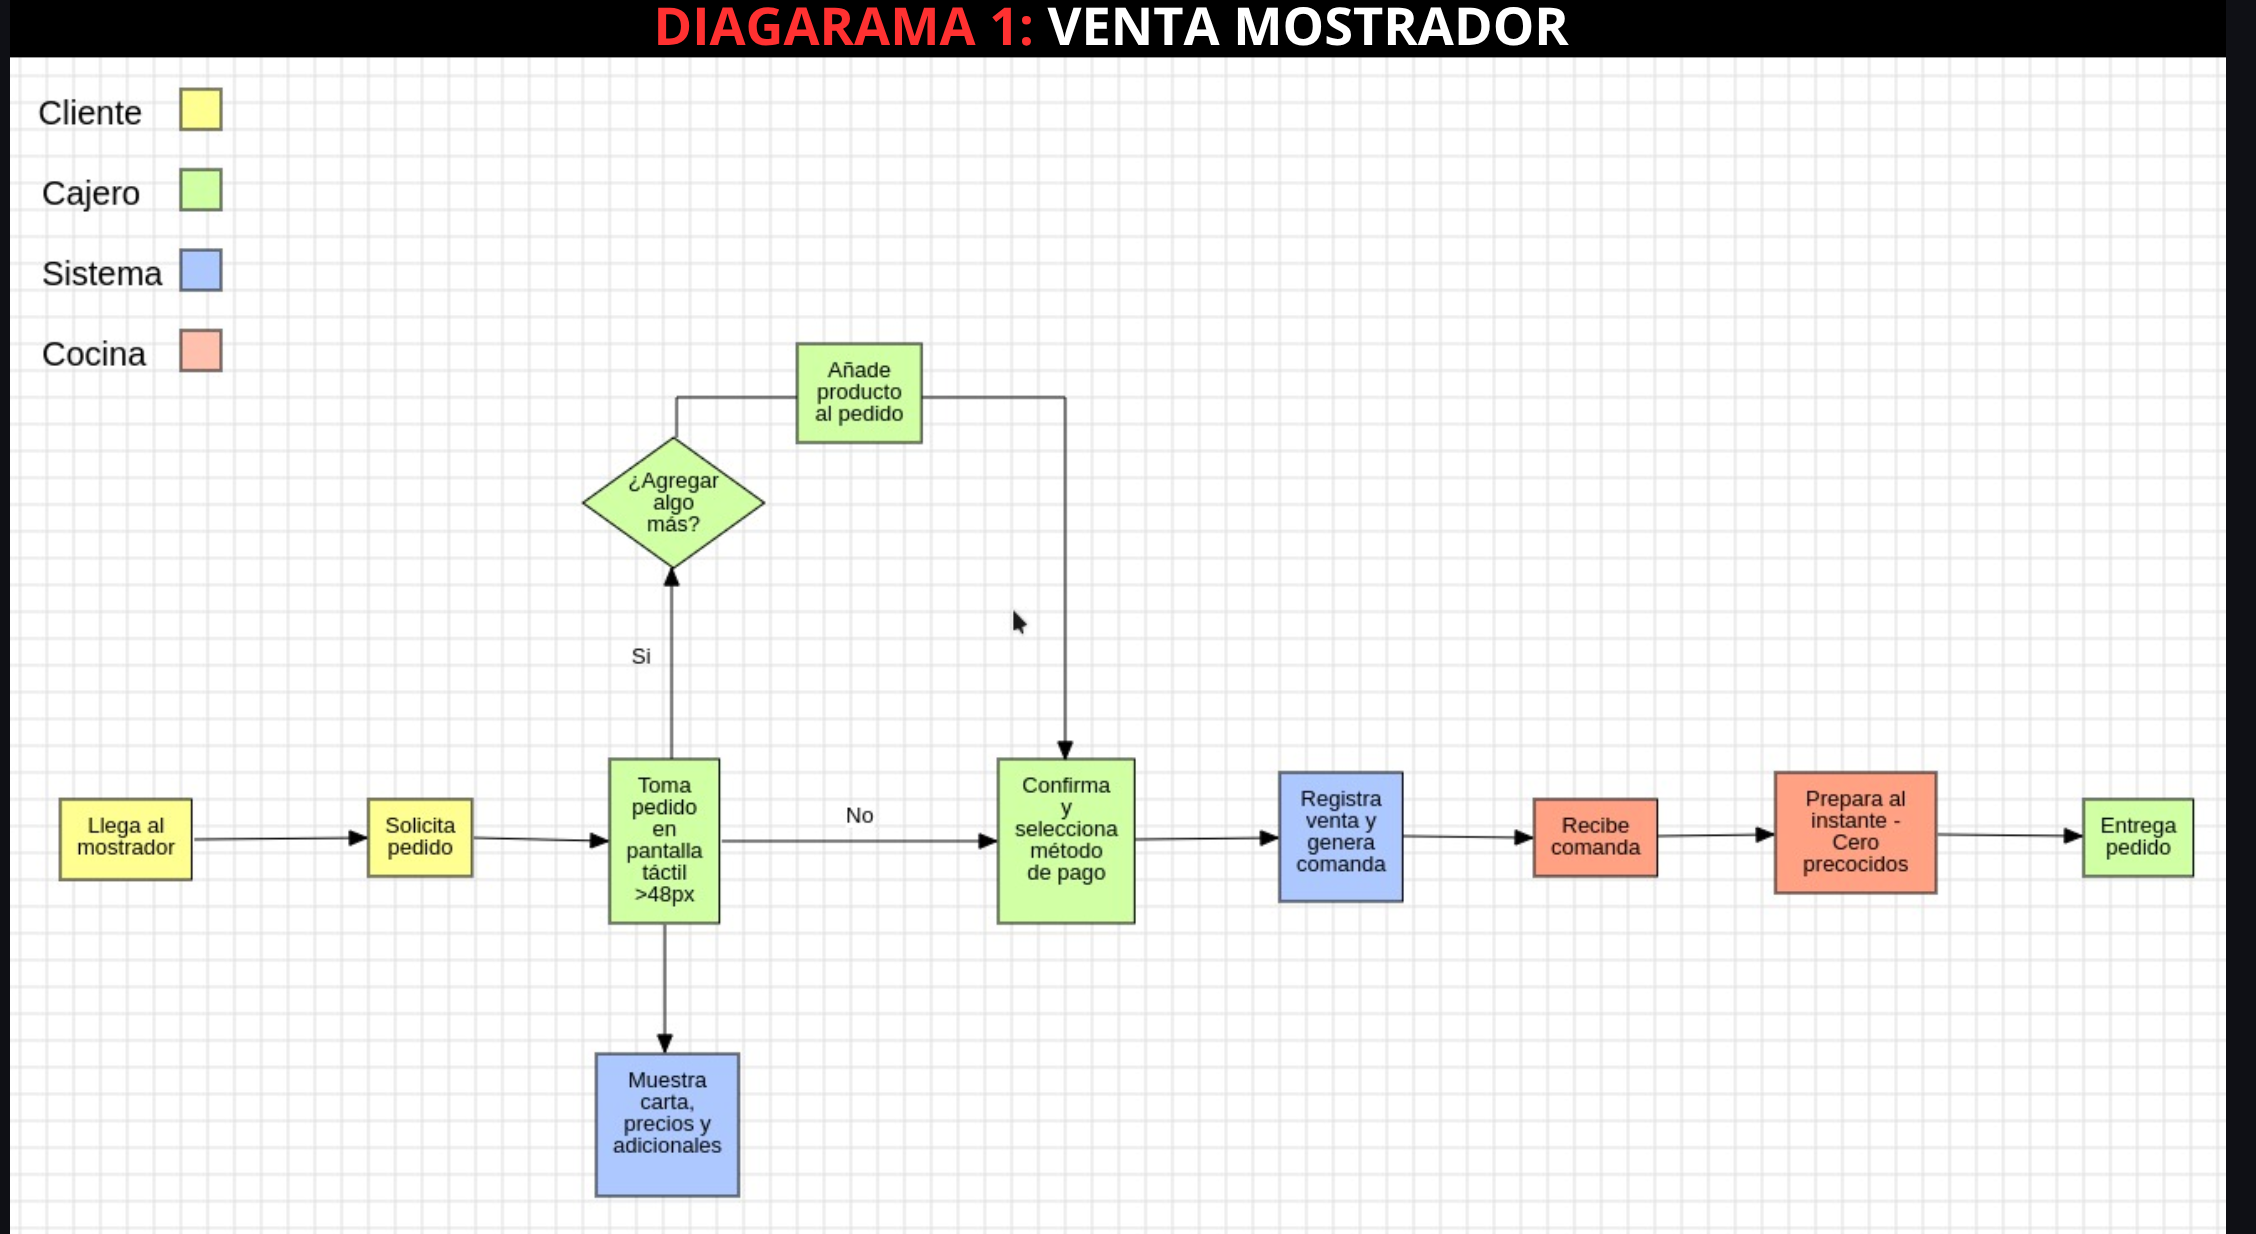
\includegraphics[width=\linewidth]{01-venta-mostrador.png}
  \caption{Diagrama 1: venta en mostrador. La caja toma el pedido en
  pantalla táctil; si el cliente agrega productos se vuelve a la carta y,
  al confirmar, el sistema registra la venta, asigna un identificador y
  genera la comanda que cocina prepara al instante.}
  \label{fig:venta-mostrador}
\end{figure}

\begin{figure}[H]
  \centering
  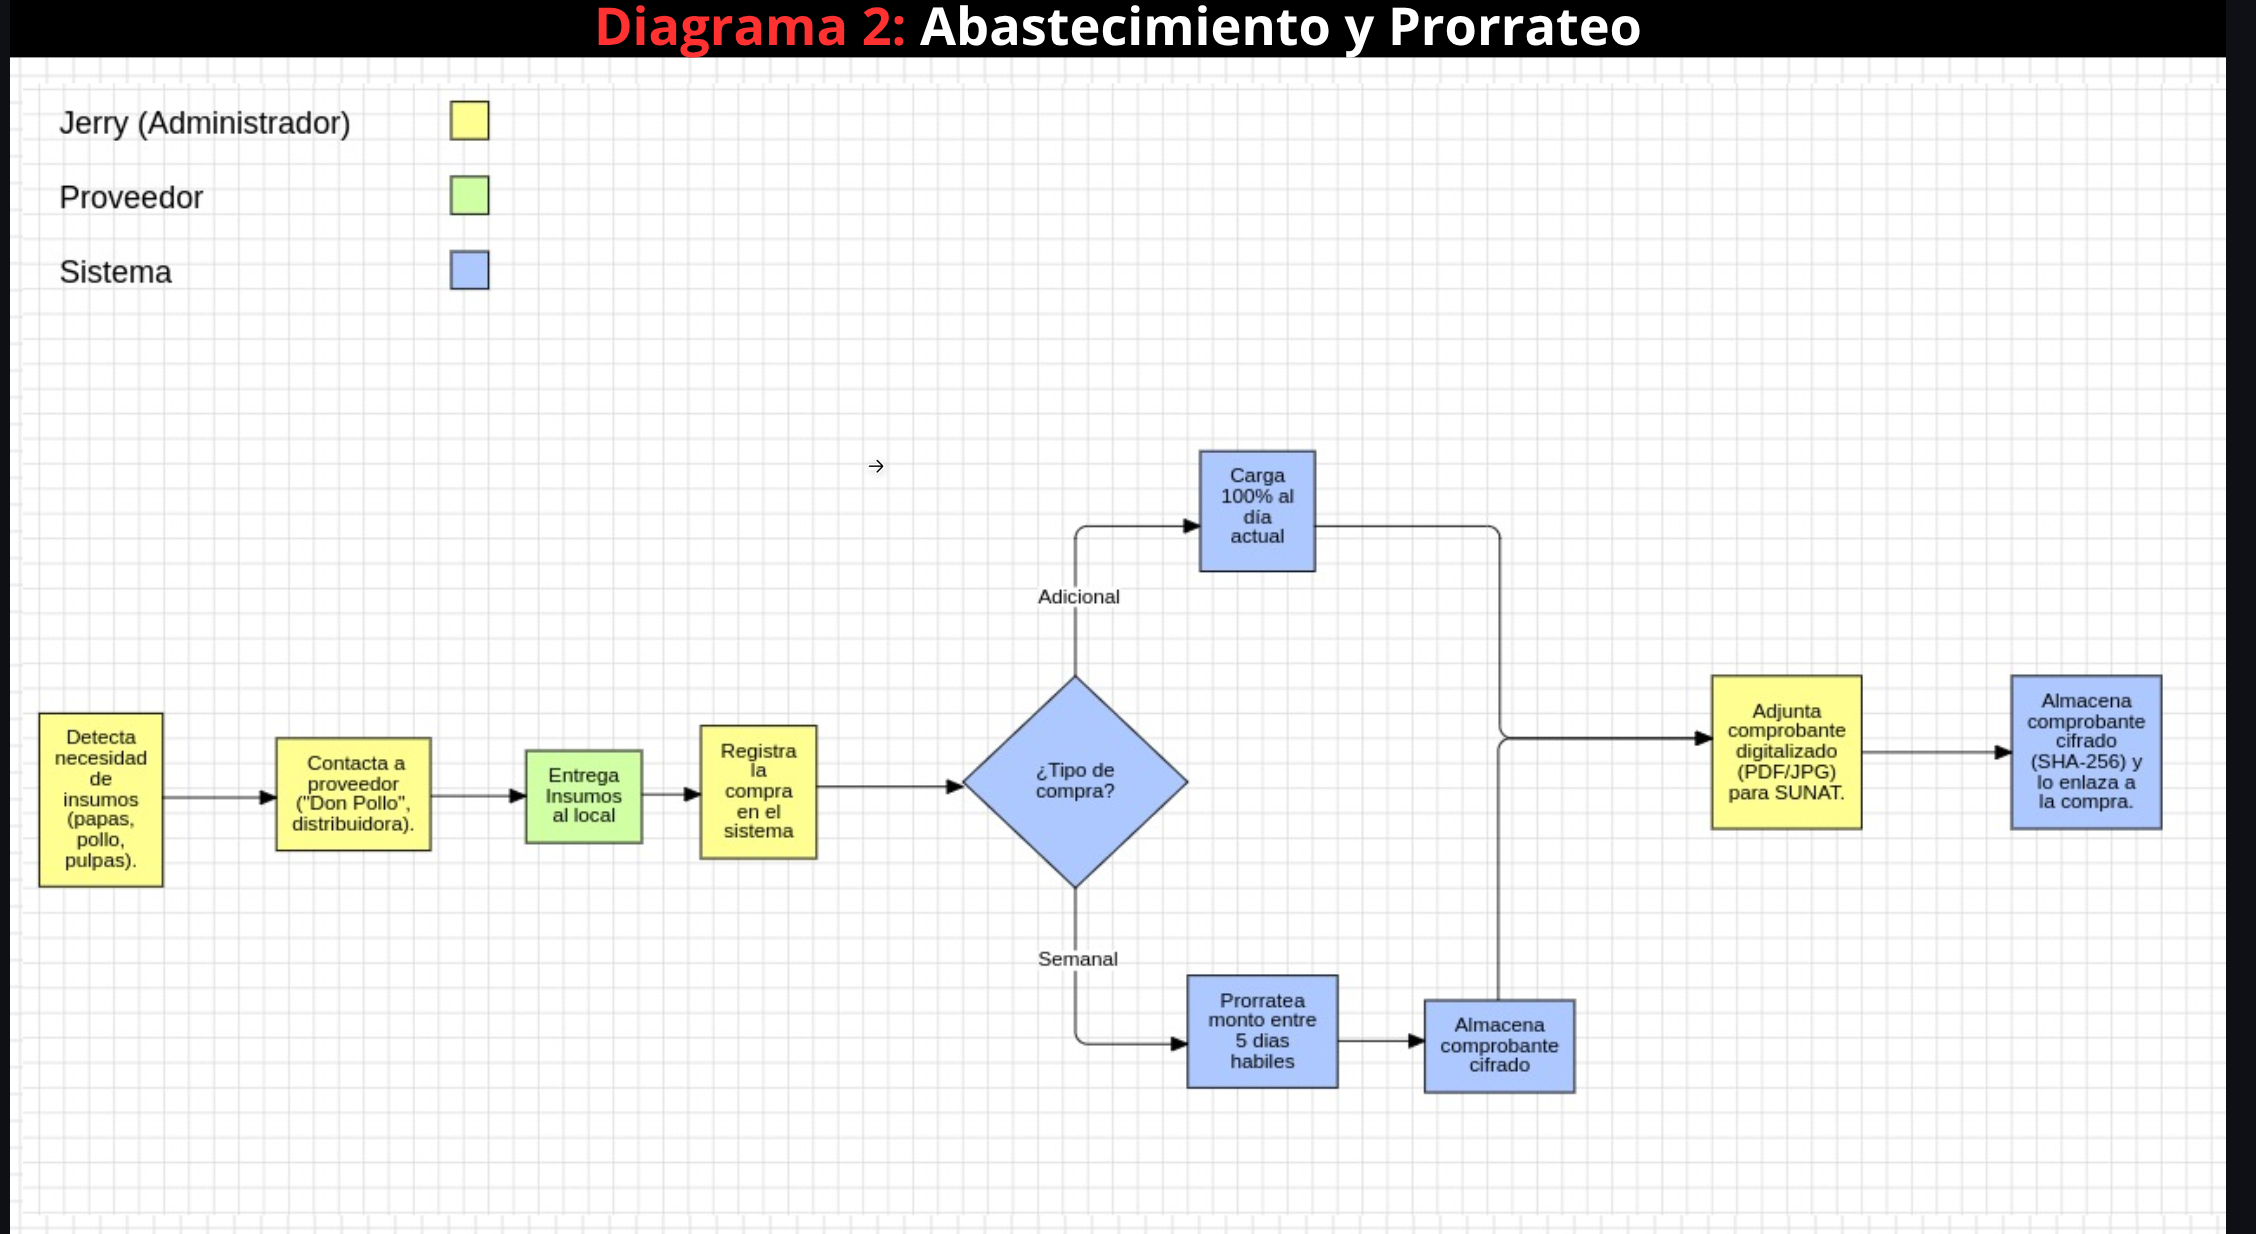
\includegraphics[width=\linewidth]{02-abastecimiento-prorrateo.png}
  \caption{Diagrama 2: abastecimiento y prorrateo. Tras registrar la compra
  se decide su tipo: la adicional se imputa al 100\,\% en la fecha de
  compra y la semanal se prorratea entre jornadas hábiles efectivas. En
  ambos casos se adjunta el comprobante, se calcula su hash SHA-256 —que
  verifica integridad, no cifra—, se cifra el archivo y se vincula al
  egreso.}
  \label{fig:abastecimiento}
\end{figure}

\begin{figure}[H]
  \centering
  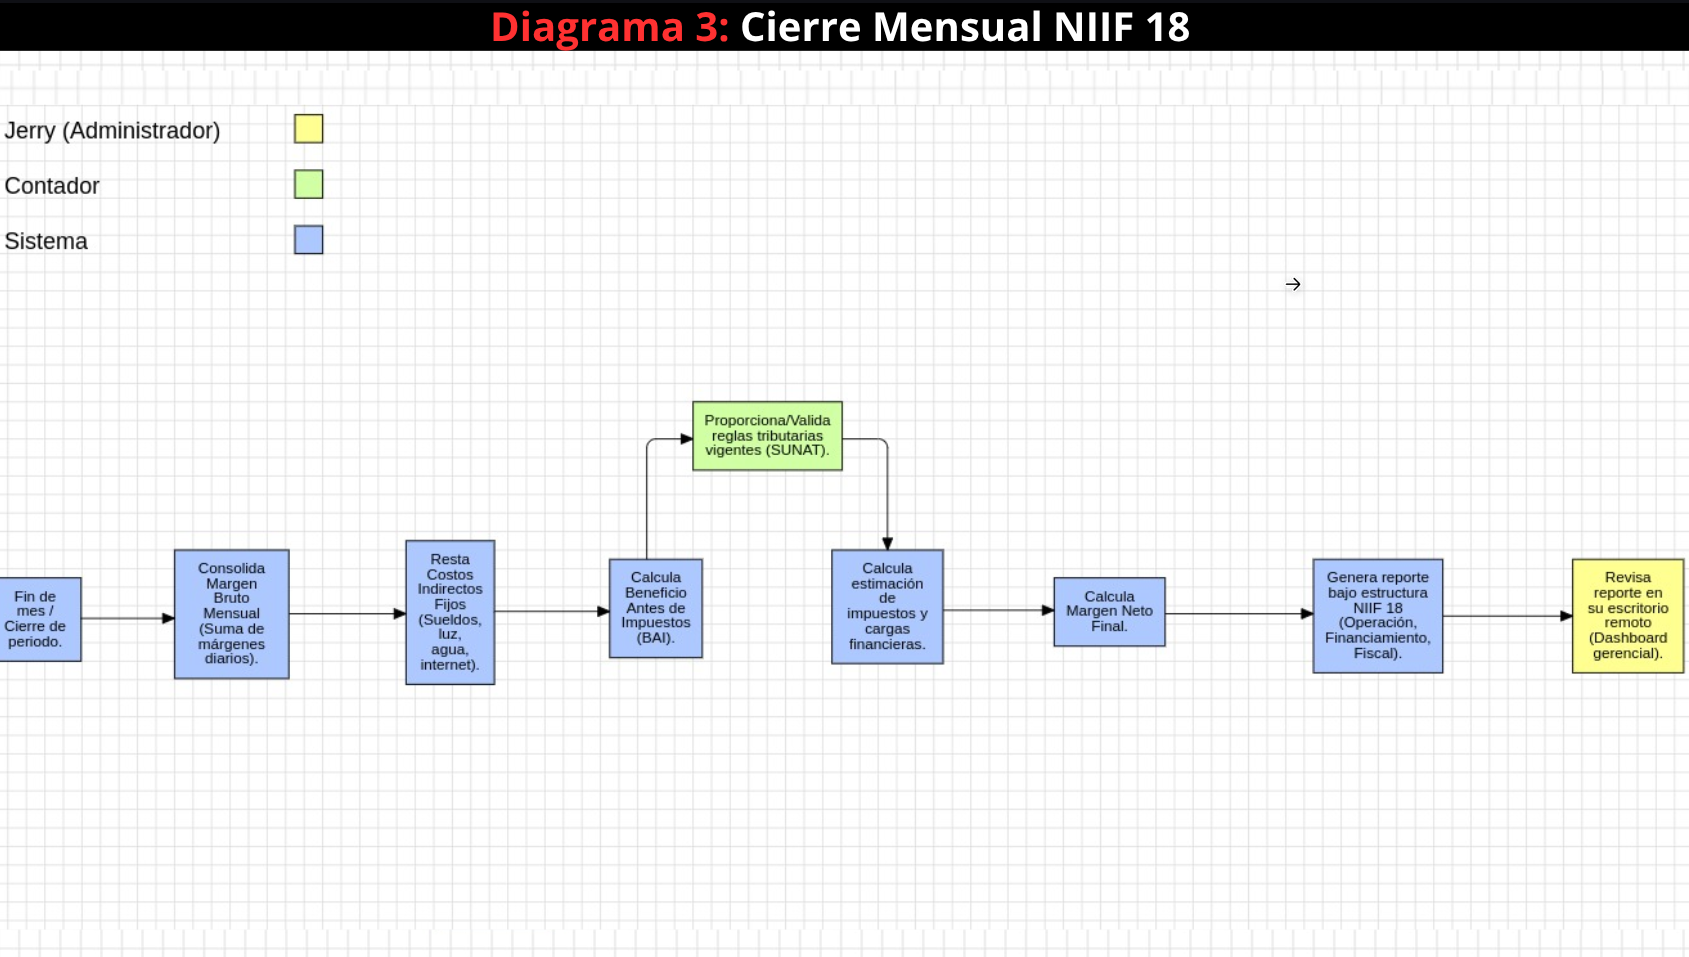
\includegraphics[width=\linewidth]{03-cierre-mensual-niif18.png}
  \caption{Diagrama 3: cierre mensual NIIF 18. Del margen bruto mensual se
  restan los costos indirectos fijos y se obtiene el resultado operativo;
  luego se deducen los gastos financieros para llegar al BAI, el contador
  valida las reglas tributarias, se calcula el impuesto a la renta y se
  llega al resultado neto, que alimenta el reporte NIIF 18.}
  \label{fig:cierre-mensual}
\end{figure}

\begin{figure}[H]
  \centering
  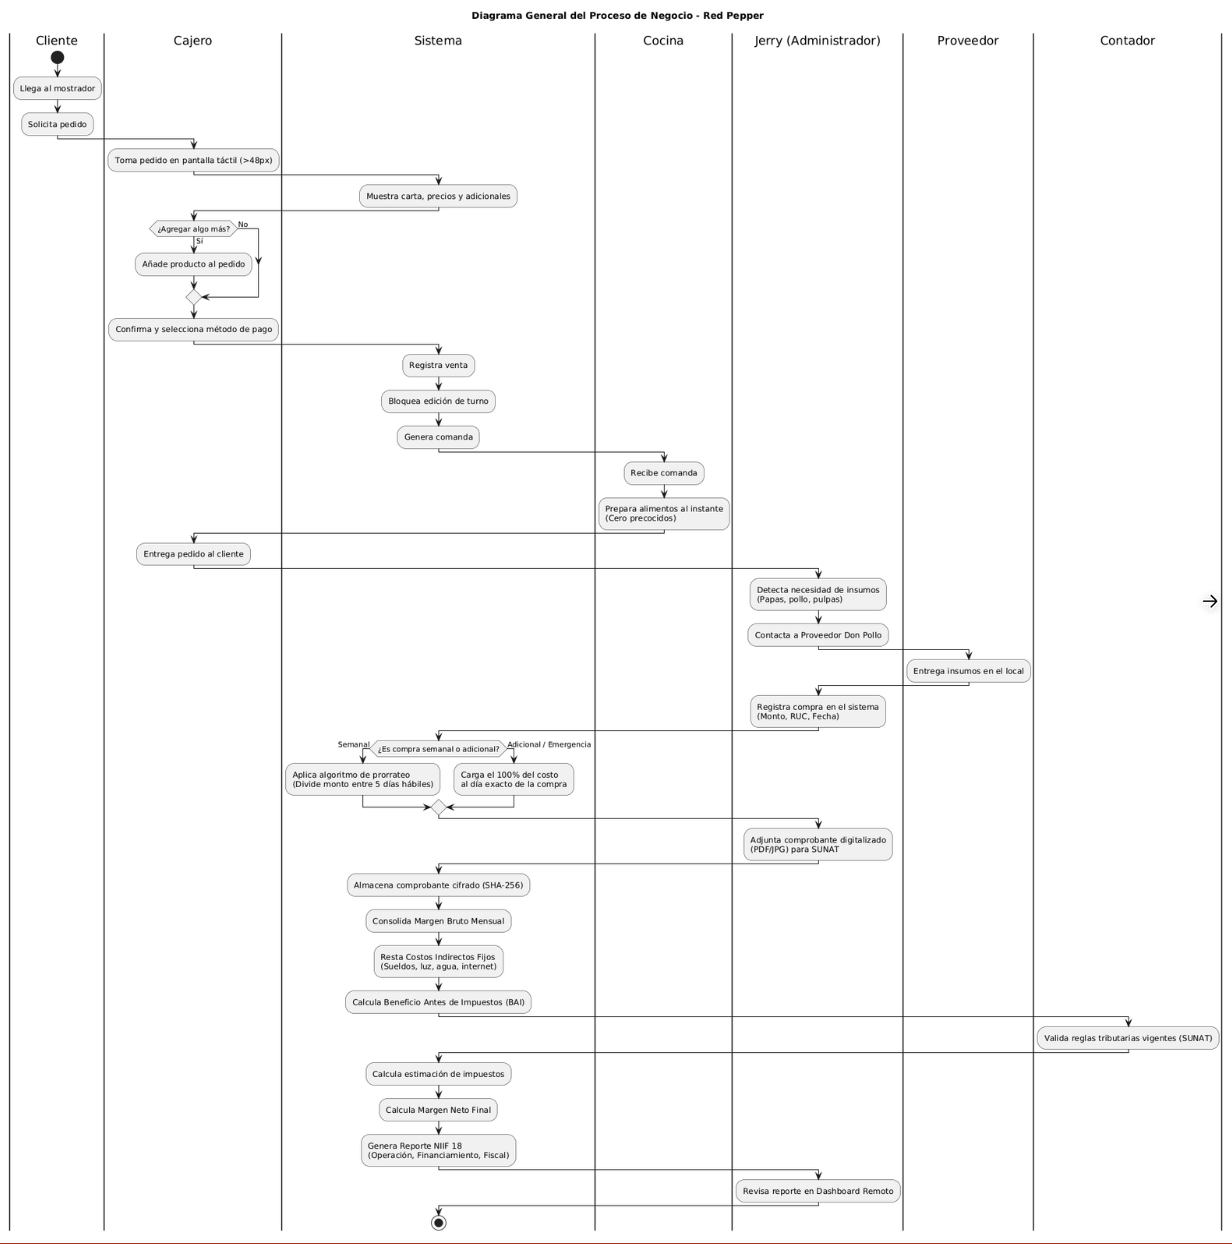
\includegraphics[width=\linewidth]{04-proceso-general.png}
  \caption{Diagrama general del proceso de negocio de RedPepper. Resume el
  negocio en tres fases encadenadas —venta en mostrador, abastecimiento con
  prorrateo y cierre mensual— y remite a los diagramas 1, 2 y 3 para el
  detalle de cada una.}
  \label{fig:proceso-general}
\end{figure}


\end{document}
